\documentclass{article}
\usepackage{graphicx}
\usepackage{ragged2e}
\usepackage{hyperref}
\usepackage{tex4ebook}
\usepackage{ifpdf}
\usepackage{float}
\usepackage{titlesec}
\usepackage{listings}
\usepackage{xcolor}

\usepackage{variables}
\titleformat{\section}[block]{\normalfont\Large\bfseries}{\thesection}{1em}{}
\titlespacing*{\section}{0pt}{\baselineskip}{\baselineskip}

\lstset{
  basicstyle=\ttfamily,
  escapeinside=||
}

\setlength{\parskip}{\baselineskip}%
\title{
  
\includegraphics[width=5cm]{Images/Logo.png}\\
  \normalsize Department of Electrical and Computer Engineering\\
  ENEL 453: Digital System Design
}

\date{\semester}

\makeatletter
\renewcommand{\maketitle}{%
  \begin{center}
    {\@title}
    \vspace{1cm} % Space between title and date, adjust as needed
    {\@date}
  \end{center}
}
\makeatother

\begin{document}
\centering

\maketitle
\large Lab 1: Introduction to Simulation, Synthesis and Implementation on an FPGA \\
\large Instruction Manual

\RaggedRight
\section{Overview}

\normalsize
\ifdefined\devinisteaching
ENEL 453 was one of my favorite courses when I took it during my undergrad. It helped inspire me towards pursuing VLSI as a field, and gained me a substantial leg up when it came to designing FPGA based systems. The reason it was as effective as it was is because I played relentlessly with the code, improving both my test benches and my designs. I encourage you to do the same, play with your designs and go beyond what the labs ask of you, I assure you it is the best way to do well in this course. 
\else
 ENEL 453 is a crucial course that can shape your understanding and enthusiasm for VLSI and FPGA-based systems. The effectiveness of this course comes from deeply engaging with the code, refining test benches, and pushing the boundaries of the lab requirements. Engaging in this manner is highly recommended for succeeding in this course.
\fi
\bigskip

\ifdefined\devinisteaching
A word of warning to students who scoff at test benches. By the end of this course your synthesis times for your FPGA may end up exceeding 1 hour. Effective test benches are the only way to complete your labs in a reasonable length of time. If you go further you may end up with synthesis times taking days to complete. Learn to make quality test benches early, and you'll save more time in the long run. 
\else
A word of warning to students who scoff at test benches. By the end of this course your synthesis times for your FPGA may end up exceeding 1 hour. Effective test benches are the only way to complete your labs in a reasonable length of time. If you go further you may end up with synthesis times taking days to complete. Learn to make quality test benches early, and you'll save more time in the long run. 
\fi
\bigskip

\ifdefined\devinisteaching
I am happy to say we are moving to one of my personal favorite FPGA boards. The Basys3 by digilent, a nifty little board with lots 
of peripherals, and a surprisingly powerful Artix 7 FPGA. The manual for the board is available here: \url{\basys3manual}. 
\else
  This course will use the Basys3 by Digilent, an excellent FPGA board that comes with a variety of peripherals and features a powerful Artix 7 FPGA. The manual for the board is available here: \url{\basys3manual}.
\fi
\vspace{0.5cm}
\\
\textbf{
This lab is worth \laboneisworth{} of your term grade and broken up as:
}
\begin{itemize}
    \item Simulations, Code, and Video Explanation: \laboneisworth
\end{itemize}
\textbf{*There will be an in-lab demonstration/ oral-examination for Lab 4.}

\section{Before You Begin}
\begin{itemize}
    \item Read through the entire lab manual before beginning on the programming
    \item \textbf{Students are working independently! All boards must be returned at the end of each lab session!}
    \item Backup your projects!
    \item Lab 2 you are only graded on your online submission, nothing in the submission needs to relate to the board.
    \item Submissions should include all of your source files and test bench files, alongside a video explaining them. 
    \item Lab 2 Simulations are due \labTwoSimsDue{}.
    
\end{itemize}

\section{Creating Vivado Projects}
\subsection{Open Vivado 2023}
    
    \ifpdf
        \begin{figure}[H]
        Open Vivado and click on Create Project under the quick start menu. 

            \centering
            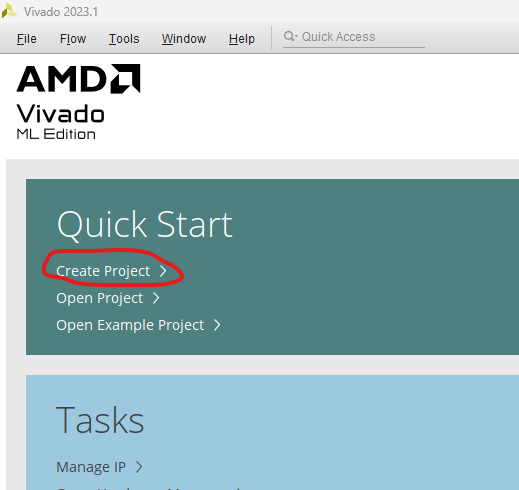
\includegraphics[width=5cm]{Images/Vivado_CreateProject.png}
            \caption{Select Create Project}
            \label{fig:enter-label}
        \end{figure}
    \else
        \HCode{<video width="320" height="240" controls>
          <source src="Images/CreateProject_Vivado2023.mp4" type="video/mp4">
          <img src="Images/Vivado_CreateProject.png" alt="Video Shows the button press for the create project">
          Your browser does not support the video tag.
        </video>}
    \fi

\subsection{Create a New Project}
    Follow along with the Create a New Project Wizard.\\
    \vspace{1cm}
    
\includegraphics[width = 1cm]{Images/Alert Icon.png} \textbf{
    If you are working on the lab computers, ensure your project is saved on your Desktop!
    This is due to file latency with the H drive preventing tools from behaving correctly.
    You will need to also ensure you backup your project as the drive gets cleaned intermittently.
    DO NOT SAVE TO THE TEMP DRIVE as that is shared between users.}

    \vspace{1cm}
    
\ifpdf
    \begin{figure}[H]
        \centering
        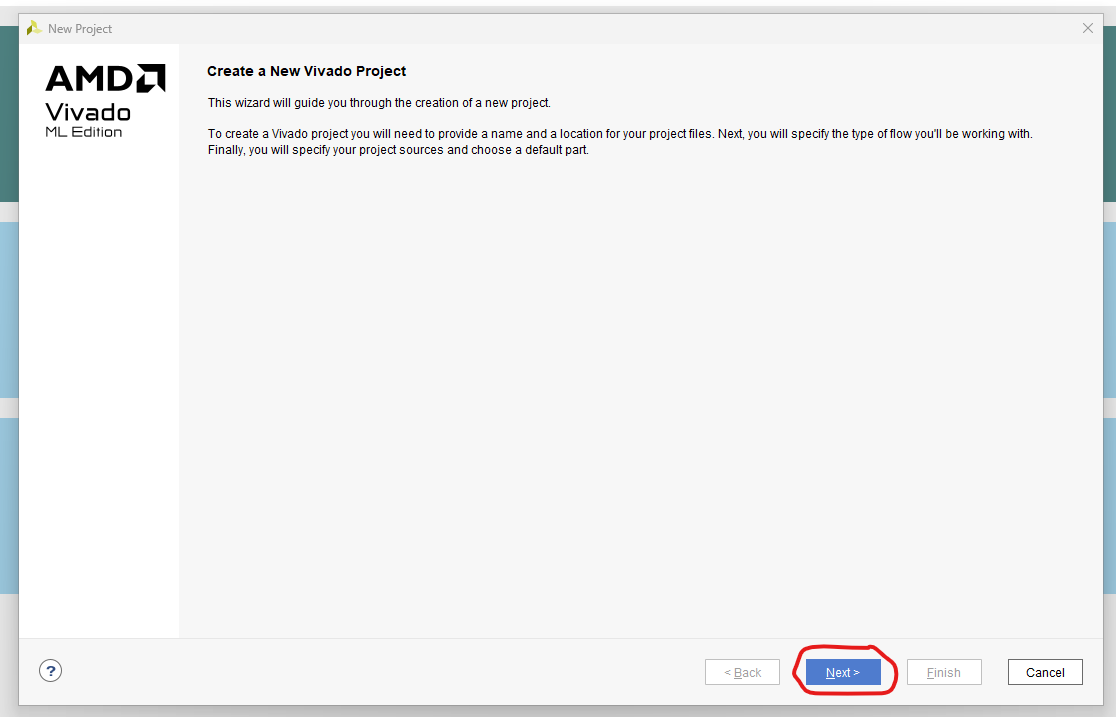
\includegraphics[width=9cm]{Images/CreateProjectImages/Vivado_CreateProject_Page1.png}
        \caption{Follow through with create project wizard.}
        \label{fig:enter-label}
    \end{figure}
    \begin{figure}[H]
        \centering
        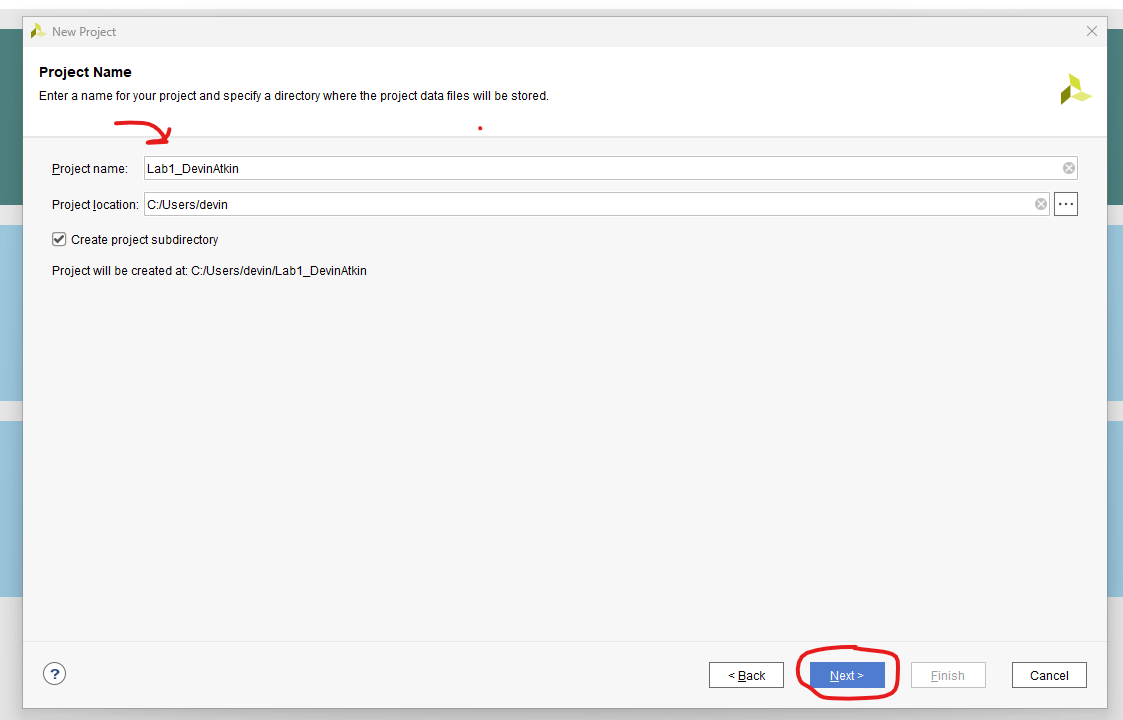
\includegraphics[width=9cm]{Images/CreateProjectImages/Vivado_CreateProject_Page2.png}
        \caption{Give  your project a name.}
        \label{fig:enter-label}
        \raggedright
        \vspace{0.5cm}
        Use the structure 
        \textbf{LabX\_FirstName\_LastName}
        for your project name. The marking will rely on the lab names so variations may cause issues with incorrect marking! 
    \end{figure}


    \begin{figure}[H]
        \centering
        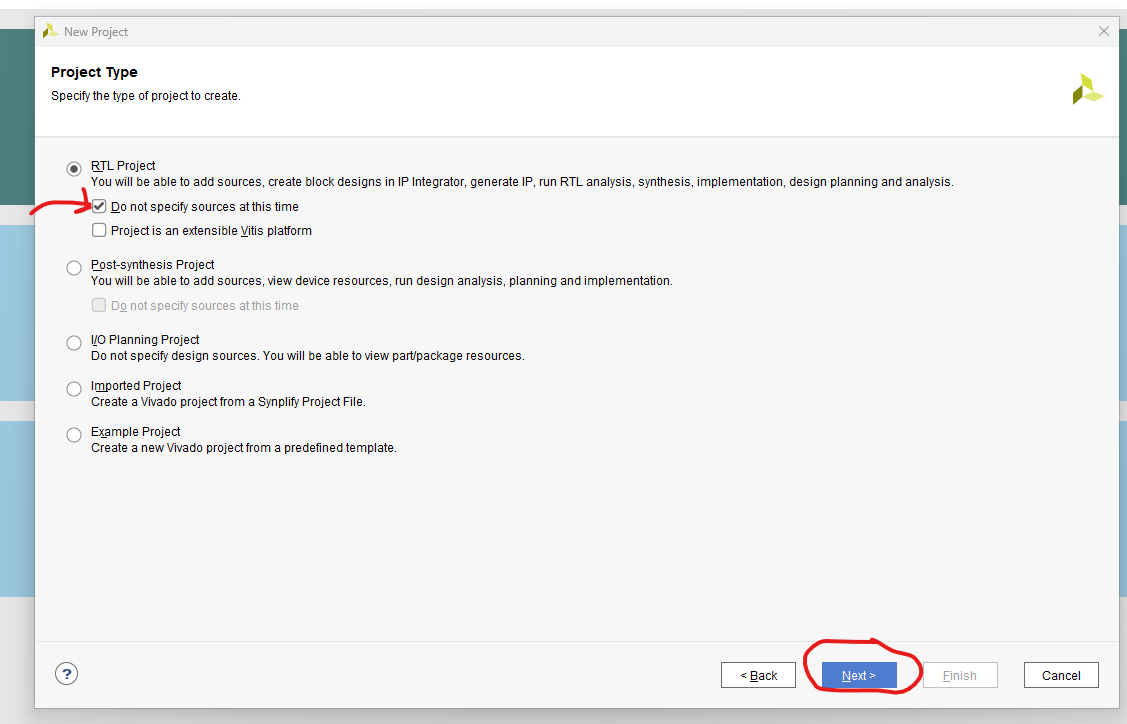
\includegraphics[width=9cm]{Images/CreateProjectImages/Vivado_CreateProject_Page3.png}
        \caption{Select RTL Project}
        \label{fig:enter-label}
        \raggedright
        Select RTL Project, and check the option to not include sources at this time. You will import the lab code once the project is fully setup.

    \end{figure}

    \begin{figure}[H]
        \centering
        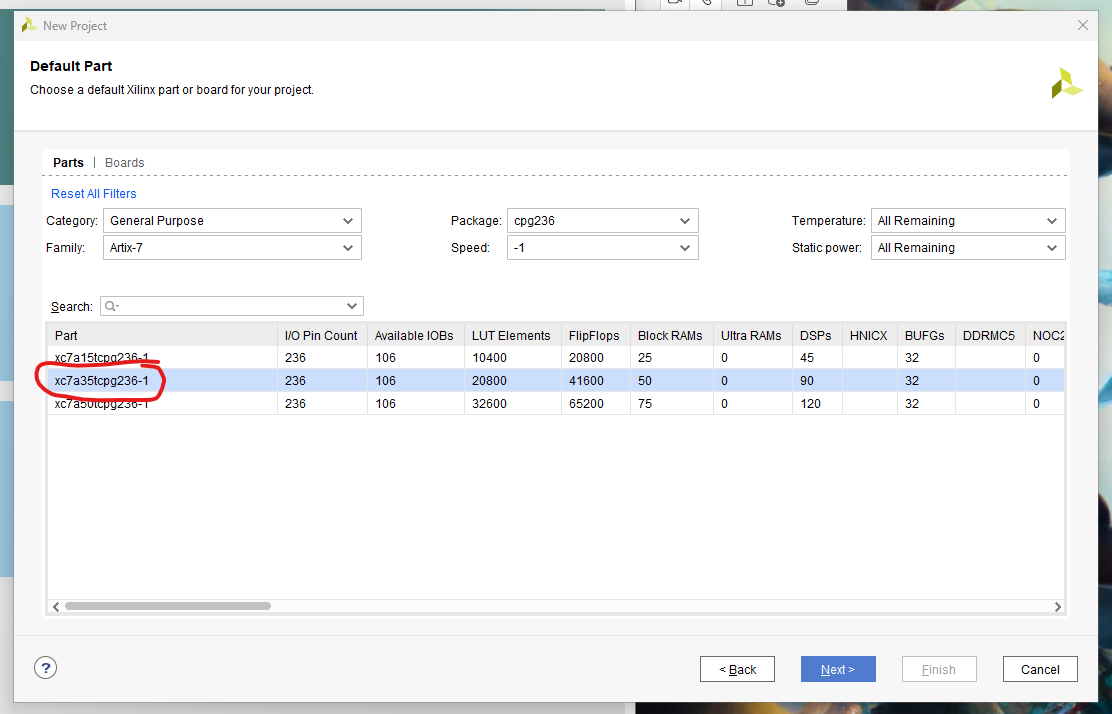
\includegraphics[width=9cm]{Images/CreateProjectImages/Vivado_CreateProject_Page4.png}
        \caption{Select the FPGA used by the Basys3}
        \label{fig:enter-label}
        \raggedright
        \vspace{0.5cm}
        The Correct FPGA is xc7a35tcpg236-1. Select the following to narrow the options.
        \begin{itemize}
            \item Category: General Purpose
            \item Family: Artix-7
            \item Package: cpg236
            \item Speed: -1
            \item Of the last 3 items in the list the center one should be correct.
        \end{itemize}
    \end{figure}
    The Basys 3 board uses an Artix-7 FPGA, selecting from the available list it is the xc7a35tcpg236-1. You can either use the search functionality or narrow the selection by choosing the appropriate category, family, package, and speed. Note that there are 3 FPGAs available with this selection, they represent different sizes of the same chip, in a design environment you would want to optimize to fit onto the smallest possible chip to minimize costs. FPGAs are expensive components; however, comparing the price of different models, the cost for the Artix-7 chips varies from ~\$50 to ~\$800. This is strong motivation to optimize your design. 

    \begin{figure}[H]
        \centering
        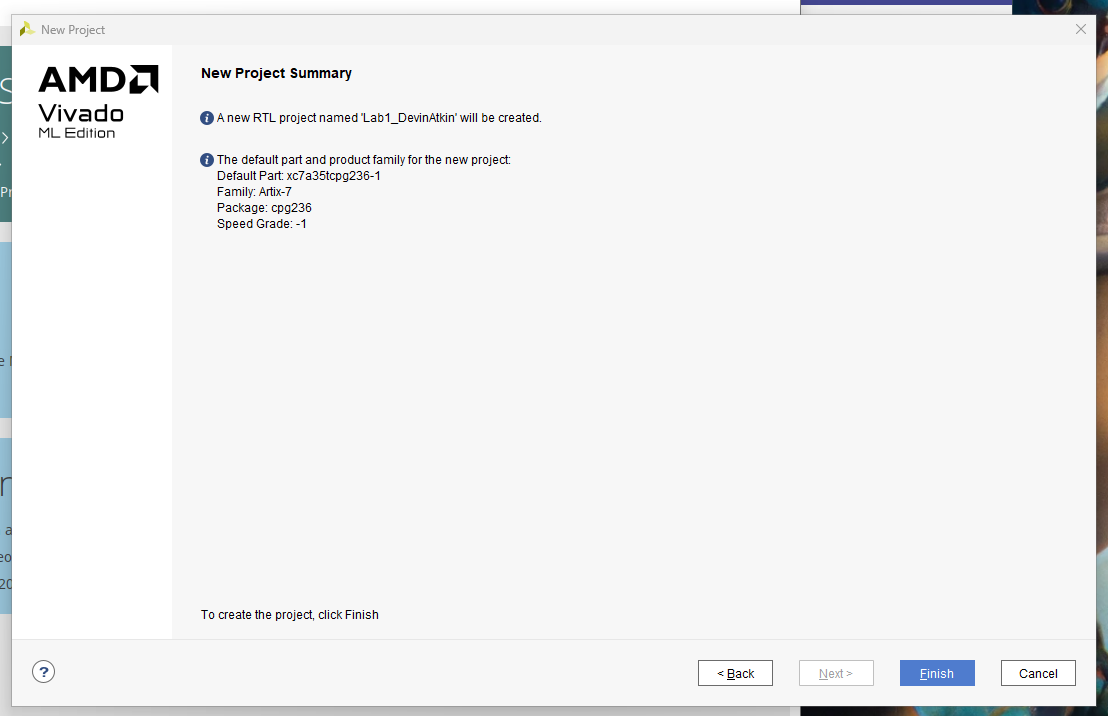
\includegraphics[width=9cm]{Images/CreateProjectImages/Vivado_CreateProject_Page5.png}
        \caption{Finish the project creation}
        \label{fig:enter-label}
    \end{figure}
    With this you should have everything setup and you can begin the lab. Verify the details listed for the project on this page and press finish to create the project. 
\else
    \HCode{<video width="320" height="240" controls>
    <source src="Images/CreateProject_Vivado2023.mp4" type="video/mp4">
    <img src="Images/Vivado_CreateProject.png" alt="Video Shows the button press for the create project">
    Your browser does not support the video tag. (Still need to update this to a new video)
    </video>}
\fi

\subsection{Adding Lab Files}
You now have a project created. You are going to need to add a handful of files to simulate and execute the project provided for this lab. The following files are provided with this lab \textit{Basys3\_Lab1\_Constraints.xdc, top\_level.sv, crc\_calc.sv, crc\_statemachine.sv, tb\_crc\_statemachine.sv, tb\_crc\_calc.sv, and tb\_top\_level.sv}. To add them to the project click on the plus sign in the sources window.

\ifpdf
    \begin{figure}[H]
        \centering
        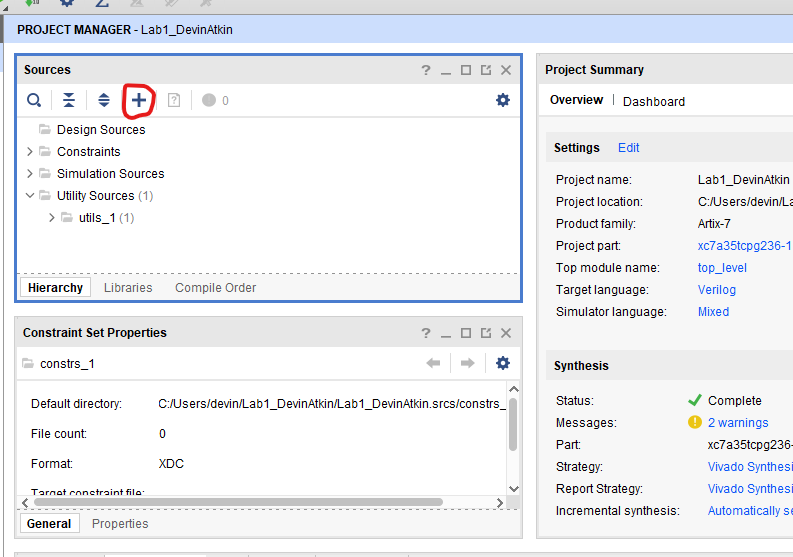
\includegraphics[width=9cm]{Images/CreateBitstreamImages/Vivado_AddSources1.png}
        \caption{Press the plus icon to begin adding sources}
        \label{fig:enter-label}
        \raggedright
        \vspace{0.5cm}
        Press the plus icon to begin adding the provided files to the project. This will bring up the add file wizard which will allow you to add each file in turn or create new files.

    \end{figure}
    
    \begin{figure}[H]
        \centering
        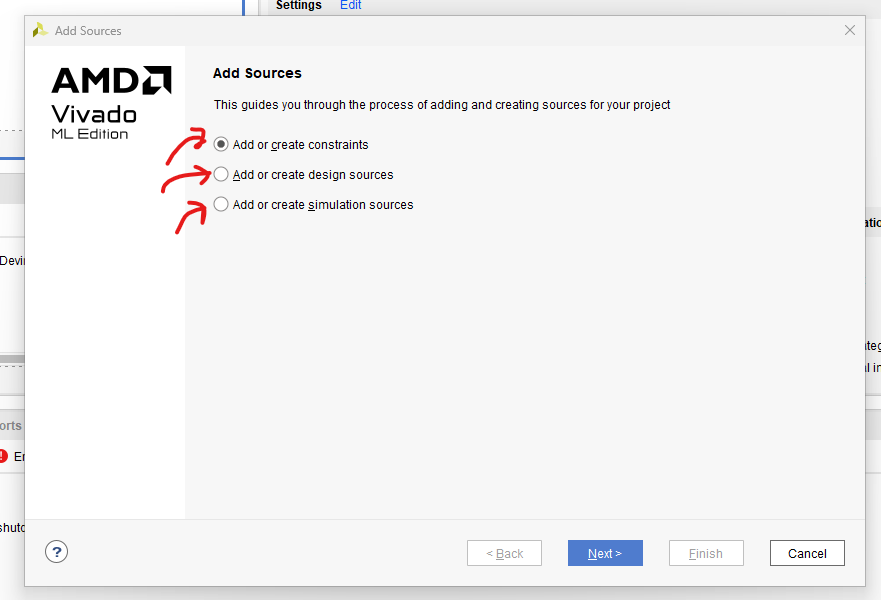
\includegraphics[width=9cm]{Images/CreateBitstreamImages/Vivado_AddSources_Page1.png}
        \caption{File Add Wizard}
        \label{fig:enter-label}
        \raggedright
        \vspace{0.5cm}
            When you press the button the Add sources tool will appear with three options.
    You'll need to repeat this step three times for the design sources (\textit{top\_level.sv, crc\_calc.sv, crc\_statemachine.sv}), simulation sources (\textit{tb\_top\_level.sv and tb\_crc\_calc.sv, tb\_crc\_statemachine.sv}), and constraints file (\textit{Basys3\_Lab1\_Constraints.xdc}). We'll explain what is in each of these files later.

    \end{figure}

    \begin{figure}[H]
        \centering
        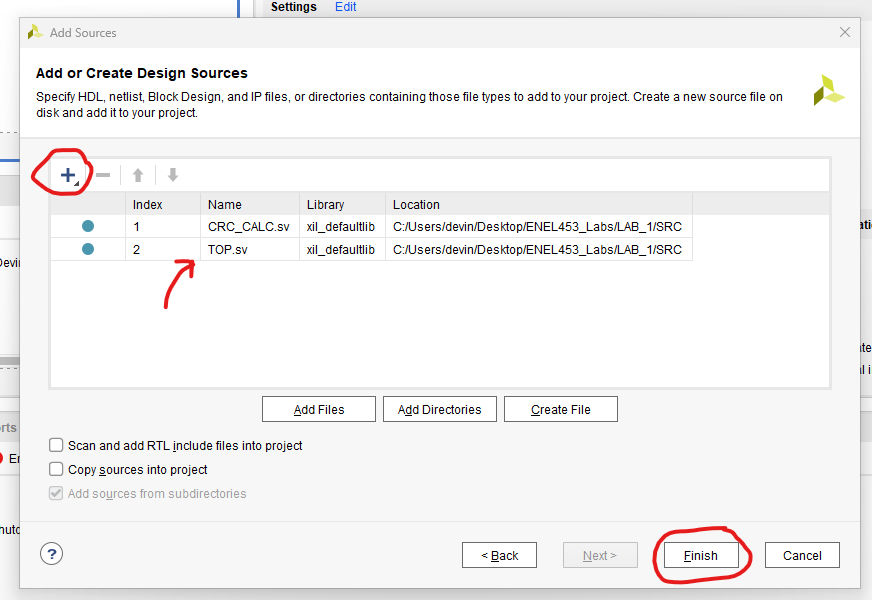
\includegraphics[width=9cm]{Images/CreateBitstreamImages/Vivado_AddSources_Page2.png}
        \caption{Select Add Files under the Plus}
        \label{fig:enter-label}
        \raggedright
        \vspace{0.5cm}
        Repeat this process for each option in turn. Hit next, select add files, and select the appropriate design sources, simulation sources, and constraints files respectively. After you have added all the provided files the design should be ready for generating a bitstream. \textbf{In the sources menu ensure that top\_level.sv is selected as the top, it will have 3 small squares next to it 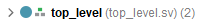
\includegraphics[height=4mm]{Images/CreateProjectImages/top_level_3Dots.png}. If it does not right click on the file in the sources menu and select Set as Top. This is the top of the design and will ensure that the bitstream is generated correctly. Vivado will often correctly select the top file when it is being added to the design. It is worth noting that top\_level or top is a fairly ubiquitous standard name for top cells in fpga projects.}
    \end{figure}

    
\else
    \HCode{<video width="320" height="240" controls>
    <source src="Images/CreateProject_Vivado2023.mp4" type="video/mp4">
    <img src="Images/Vivado_CreateProject.png" alt="Video Shows the button press for the create project">
    Your browser does not support the video tag. (Still need to update this to a new video)
    </video>}
\fi

\subsection{RTL View}
After adding your files you can check that the design is loaded correctly by opening up the RTL view. This represents your design
\begin{figure}[H]
    \centering
    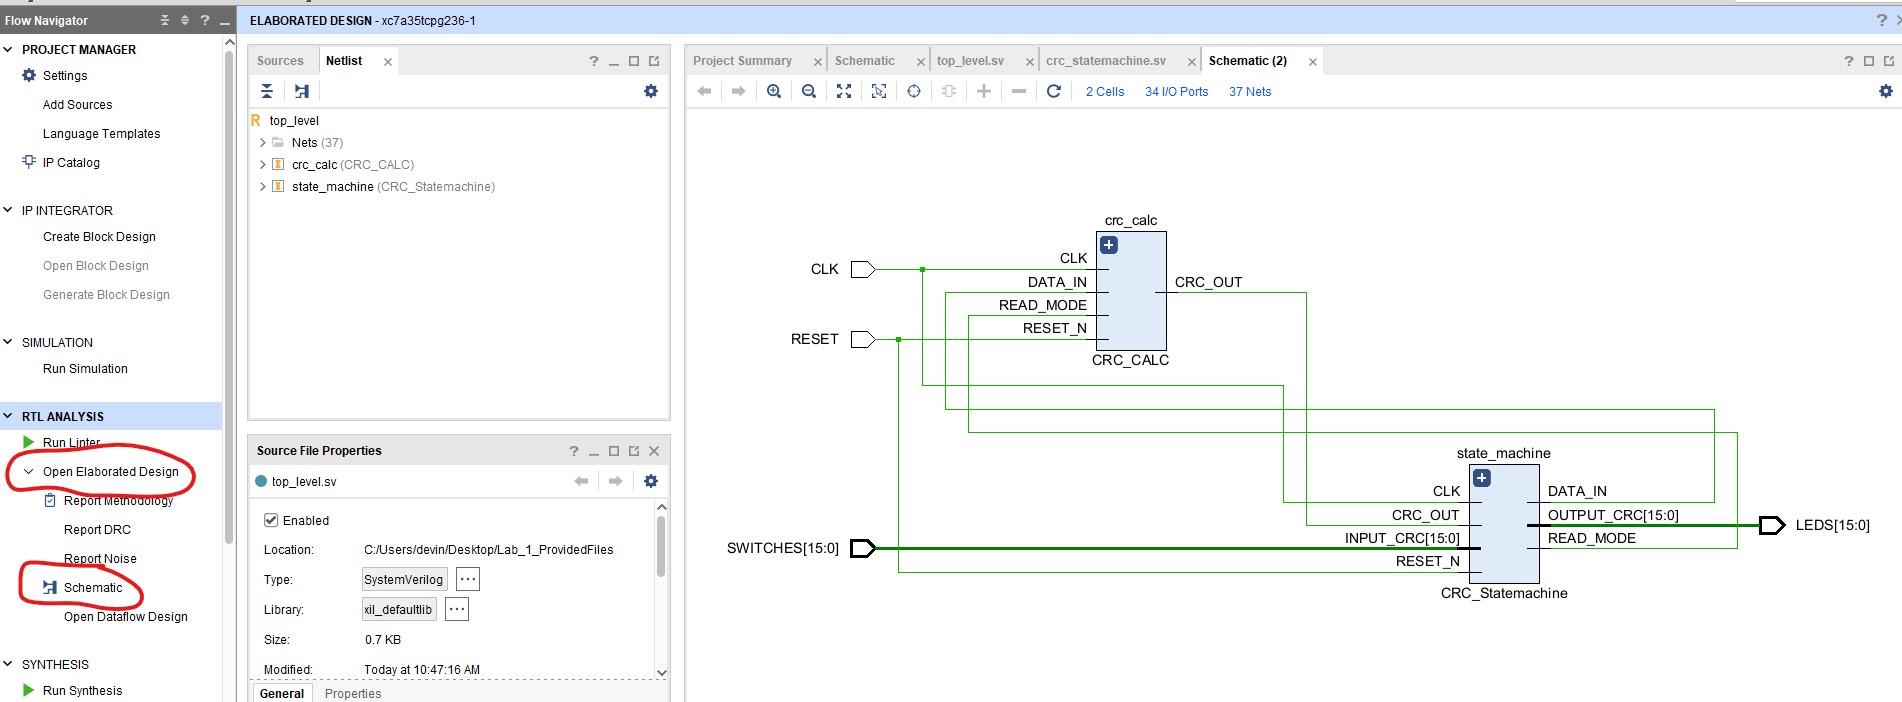
\includegraphics[width = 9cm] {Images/CreateBitstreamImages/OpenElaboratedDesign.jpg}
    \caption{Look at the RTL View}
    \label{fig:enter-label}
    \raggedright
    \vspace{0.5cm}
    Open the elaborated schematic by clicking open elaborated design, then clicking on schematic. This will compile the top level files and create a schematic representation of the design.
    You can click on the blocks in the design and it will expand out to show you the lower levels. Once finished with this lab \textbf{return to this view and include a screenshot in your design report.} Take note that no logic exists in this top level. While technically possible to have logic at any level, it is considered especially bad practice, the most logic that is considered acceptable is singular inverters. You'll need to add this to the design as part of the modifications in a later section. \\
    \vspace{0.5cm}
    
\includegraphics[height=1cm]{Images/Alert Icon.png}  \textbf{RTL view is one of the most useful tools for diagnosing problems in your FPGA design.} The RTL view represents the schematic view of your design, it is incredibly useful for confirming that you are creating the design as intended. When debugging larger designs it can be often worth restructuring larger elements to create blocks which have clear representations in the RTL view so that you can more easily diagnose issues. 
\end{figure}
\subsection{Synthesis and Implementation}
You'll remember that synthesis takes the HDL design and converts it into elements in the fpga, and then implementation takes those and maps it onto the actual fpga hardware.
\vspace{0.5cm}
\begin{figure}[H]
    \centering
    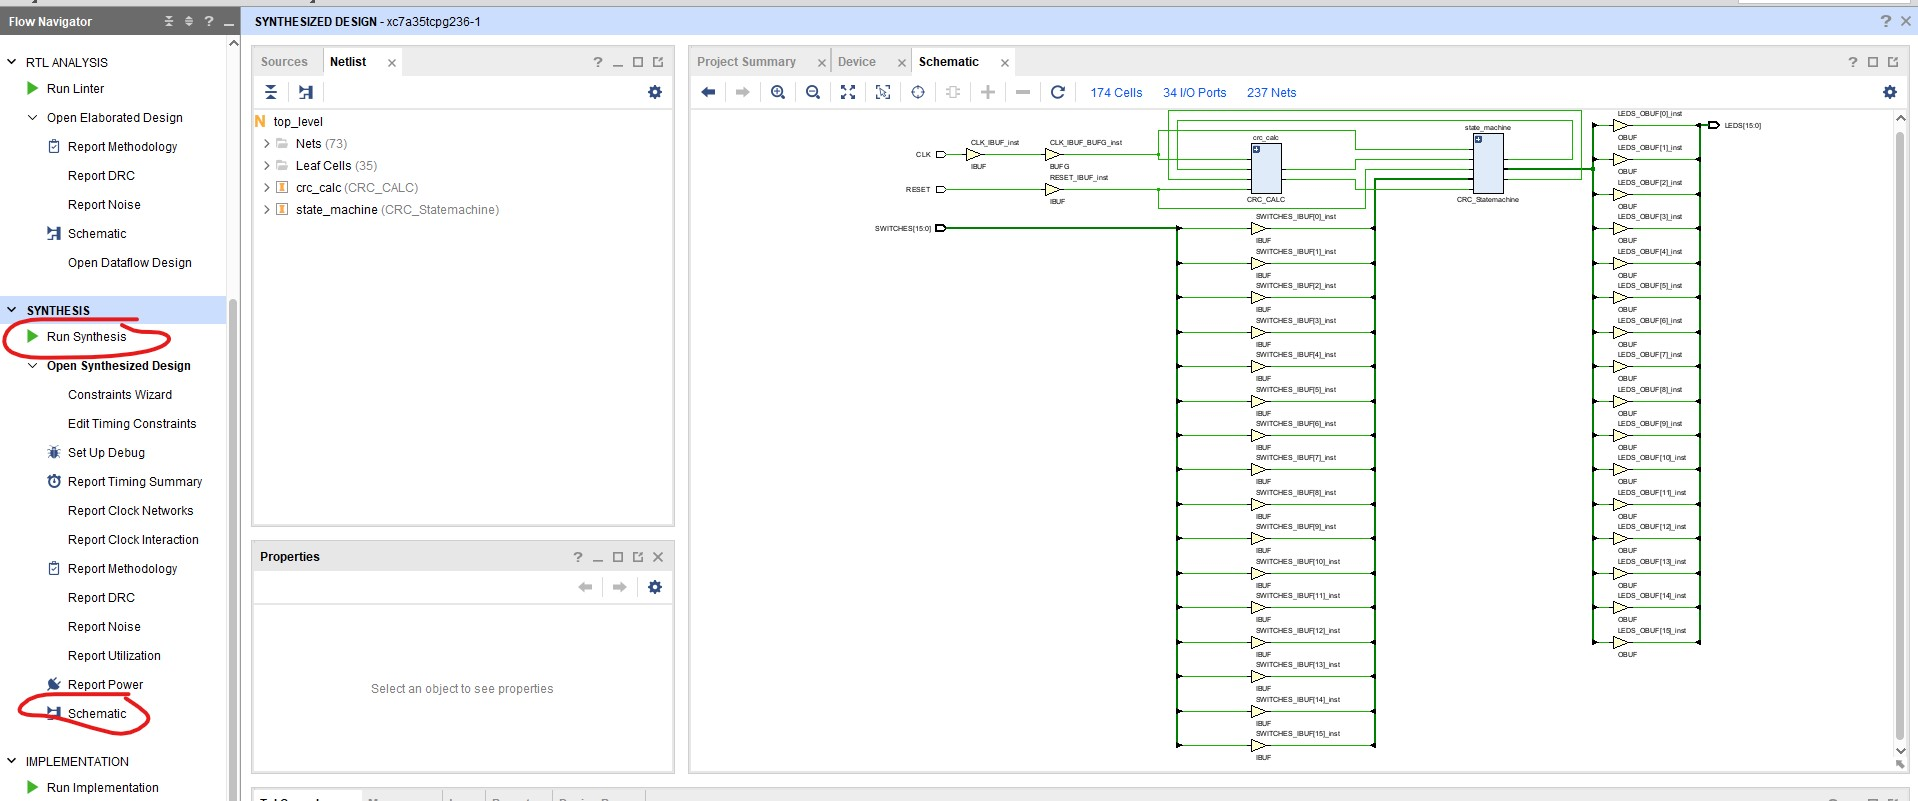
\includegraphics[width=9cm]{Images/CreateProjectImages/SynthesizeYourDesign.jpg}
    \caption{Run Synthesis}
    \label{fig:enter-label}
    \raggedright
    \vspace{0.5cm}
    Press Run Synthesis in the left hand panel. This will being up a dialog for starting synthesis, you go ahead and accept this immediately or change the number of jobs. It won't make a substantial difference in time now; however, on larger designs this will help speed up the process. Once you've run synthesis open the synthesized design and look at the schematic again, you'll notice that the logic gates have been replaced with LUTs.
\end{figure}

Once you're done looking at the elaborated design you'll want to run implementation. This will map the hardware onto the physical FPGA. This is where you'll need to grab your timing details.\\
\subsection{Implementation}
\begin{figure}[H]
    \centering
    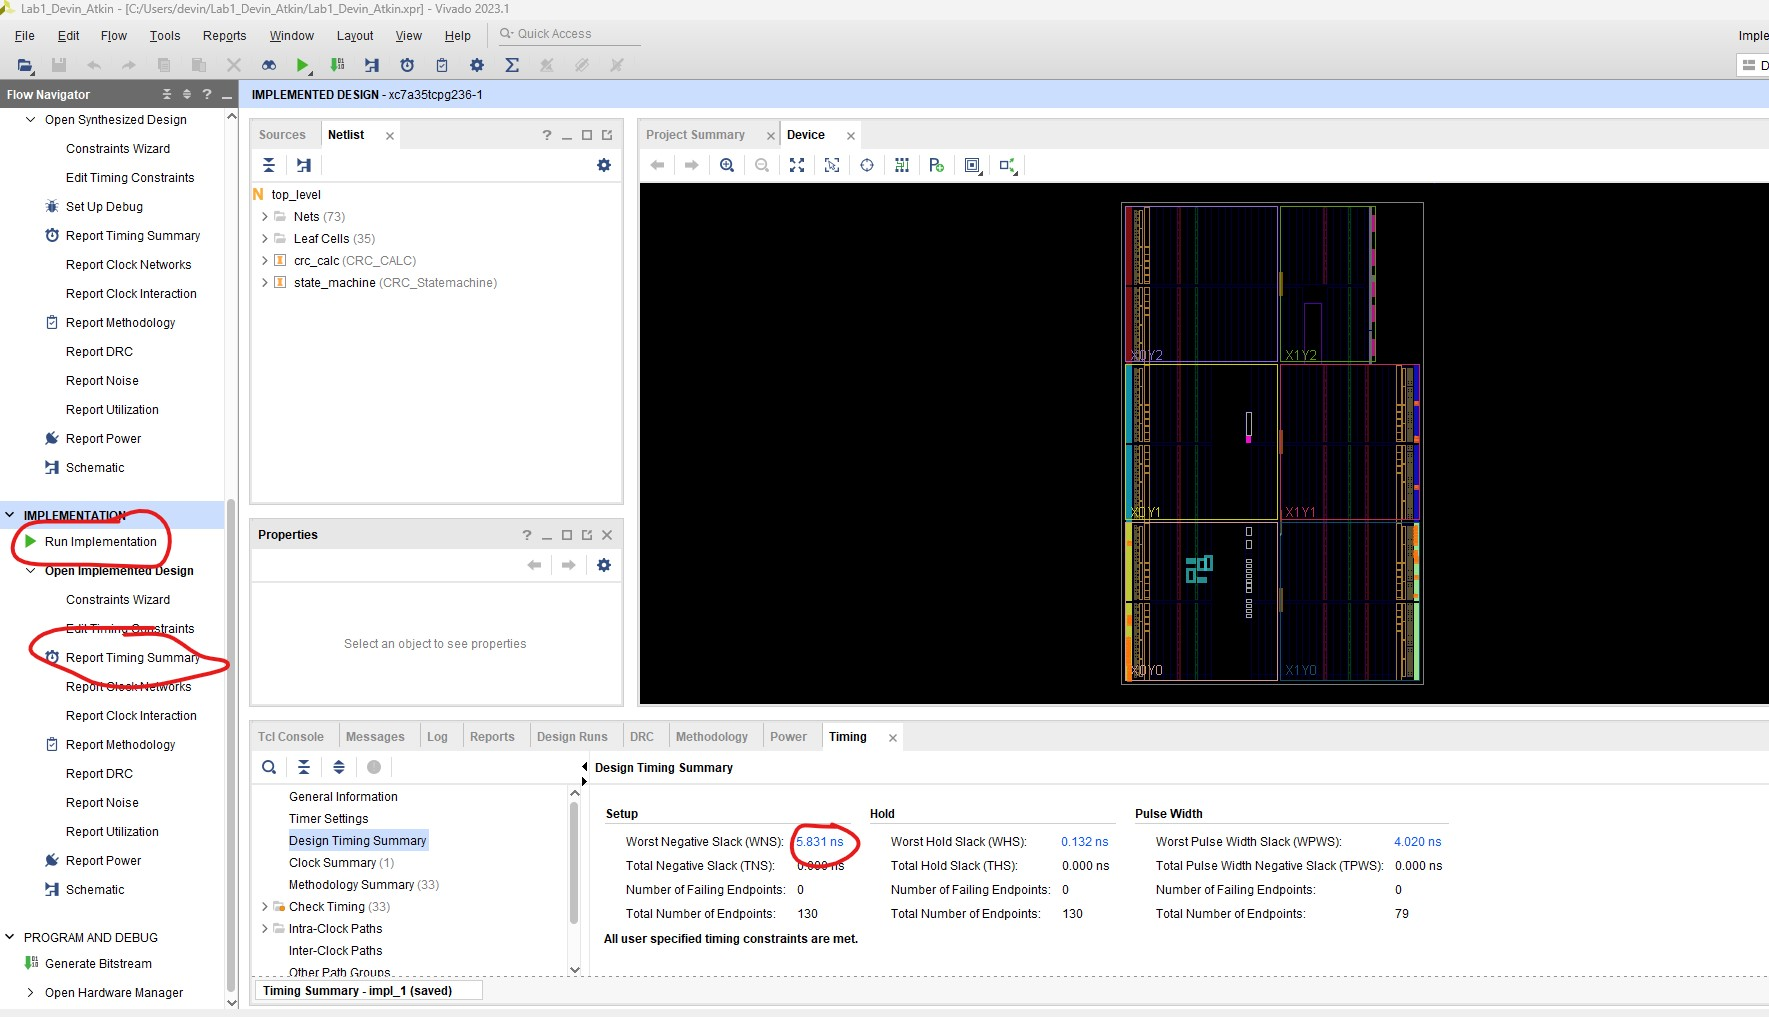
\includegraphics[width=9cm]{Images/CreateProjectImages/Implementation.jpg}
    \caption{Make sure to include your timing summary}
    \label{fig:enter-label}
\end{figure}
You will need to include the timing details on your lab design reports. You get this from the implementation. The timing summary should come up after implemention is run assuming you open the implemented design; however, if it doesn't you can get the timing summary by clicking \textit{Report Timing Summary} and then clicking ok for the default report. To Note, there is a separate timing report at the synthesis level which you don't necessarily need to pay attention to; however, if it fails to pass, implementation will almost definitely also fail to pass as well. 

\vspace{1cm}
\textbf{All of your designs must pass timing}. This means that they must be able to run at at least the 100MHz built in clock used by the Basys3. You are unlikely to run into timing issues on labs 1 and 2; however, this may become a challenge on labs 3 and 4 if you aren't careful when it comes to doing math. 

\vspace{0.5cm}
Use the following equation to calculate the maximum operating frequency for your design.
\[f_{max} = \frac{1}{t_{per}-t_{wns}} \]
Where \(f_{max}\) is the maximum operating frequency, \(t_{per}\) is the target period (in this case 10ns), and \(t_{wns}\) is the worst negative slack for the given implementation. The target period is determined by the clock speed of the design, this is defined in the constraints file for the project. You can see the clock being created here:

\begin{small}
\begin{verbatim}
## Clock signal
set_property PACKAGE_PIN W5 [get_ports CLK]							
set_property IOSTANDARD LVCMOS33 [get_ports CLK]
create_clock -add -name sys_clk_pin -period 10.00 -waveform {0 5} [get_ports CLK]
\end{verbatim}
\end{small}
The period is after the -period and is expressed in nanoseconds. However, this is determined by the crystal oscillator on the Basys3. If we were performing logic which required a slower clock speed, we would have to use either clock dividers or a PLL on chip to generate the alternate frequency. 



\section{Explaining CRC Coding and Modifying the Provided Code}

CRC stands for Cyclic Redundancy Check, it is a number which is calculated before transmitting which is appended to the message to allow to reciever to check for errors in the bit pattern. The provided code is implements a CRC check based on the switches. You can see the output by pressing the center button on the Basys 3 and toggling some of the switches. The Leds should change in what appears to be a mostly random pattern. The pattern is the calculated CRC. \\

\vspace{1cm}
To get a solid understanding of CRC I recommend watching the following videos by Ben Eater explaining the math and hardware of CRC check. The provided code implements the same standard as he implements in his video.
\begin{itemize}
    \item How do CRCs work?: \url{https://www.youtube.com/watch?v=izG7qT0EpBw}
    \item Hardware CRC calculation: \url{https://www.youtube.com/watch?v=sNkERQlK8j8}
\end{itemize}

The essential idea of a CRC check is that you guarantee your message is divisible by a specific number and then you calculate the remainder to see if the received message is correct. The specific number is typically a large prime number to ensure that it is unlikely the error which occurs results in another valid transmitted message. Selecting a good number is essential, a lab exists which maintains a list of good options for CRC values \url{https://users.ece.cmu.edu/~koopman/crc/index.html}. In our instance XMODEM which is implemented by the provided code uses 4129 which is the 519th prime number. 

While calculating a true CRC is done using XOR operations in binary, for convenience we can see the overall idea by performing the calculations mostly in decimal. We'll send "Hi" using the CRC-16 XMODEM.
\begin{itemize}
    \item We first want to look at the binary representation of the text. 01001000 01101001. 
    \item We are going to want to pad our message with an additional 16-bits to contain the calculated CRC as the final message includes the CRC: 00000000 00000000.
    \item Then lets look at the decimal representation with the padding: 1214840832.
    \item Then we are going to want to find the remainder when divided by 4129 (Our prime number): 2323
    \item If we subtract the remainder from the prime number we get 4129-2323=1806.
    \item We are then going to add that to our original number to get: 1214842638
    \item Which in decimal is 1214842638. This number is now evenly divisible by 4129 and is therefore valid. If we transmit this and an error occurs, we can know by checking if the received value is divisible by the agreed upon number (4129).
    \item If we look at the message in binary you can see the original message is still present: 01001000 01101001 00000111 00001110.

\textbf{This does give a different value than the true CRC but is a overall representation of the math in a decimal format}. True CRC calculation utilizes finite fields, and polynomial division to represent the input and output, turning the CRC calculation from a division into a series of exclusive or operations. 
\end{itemize}

\subsection{Simulating Your Designs}
We have provided functional test benches for both the top level module and the lower level CRC calculator. This works for now; however, to verify your results before submitting you will want to simulate them. Make sure that the CRC Testbench is setup as the top level simulator.

\begin{figure}[H]
    \centering
    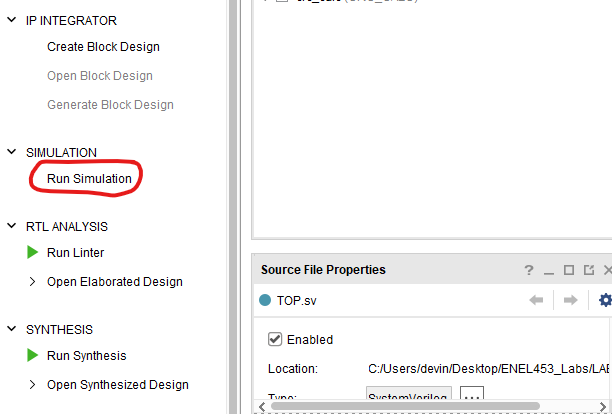
\includegraphics[width=7cm]{Images/SimulatingDesign/Run_Simulation_Page1.png}
    \caption{Press Run Simulation and select Run Behavioral Simulation}
    \label{fig:enter-label}
\end{figure}
To simulate the CRC Code calculator select Run Simulation on the side, then select run behavioral simulation. 
\begin{figure}[H]
    \centering
    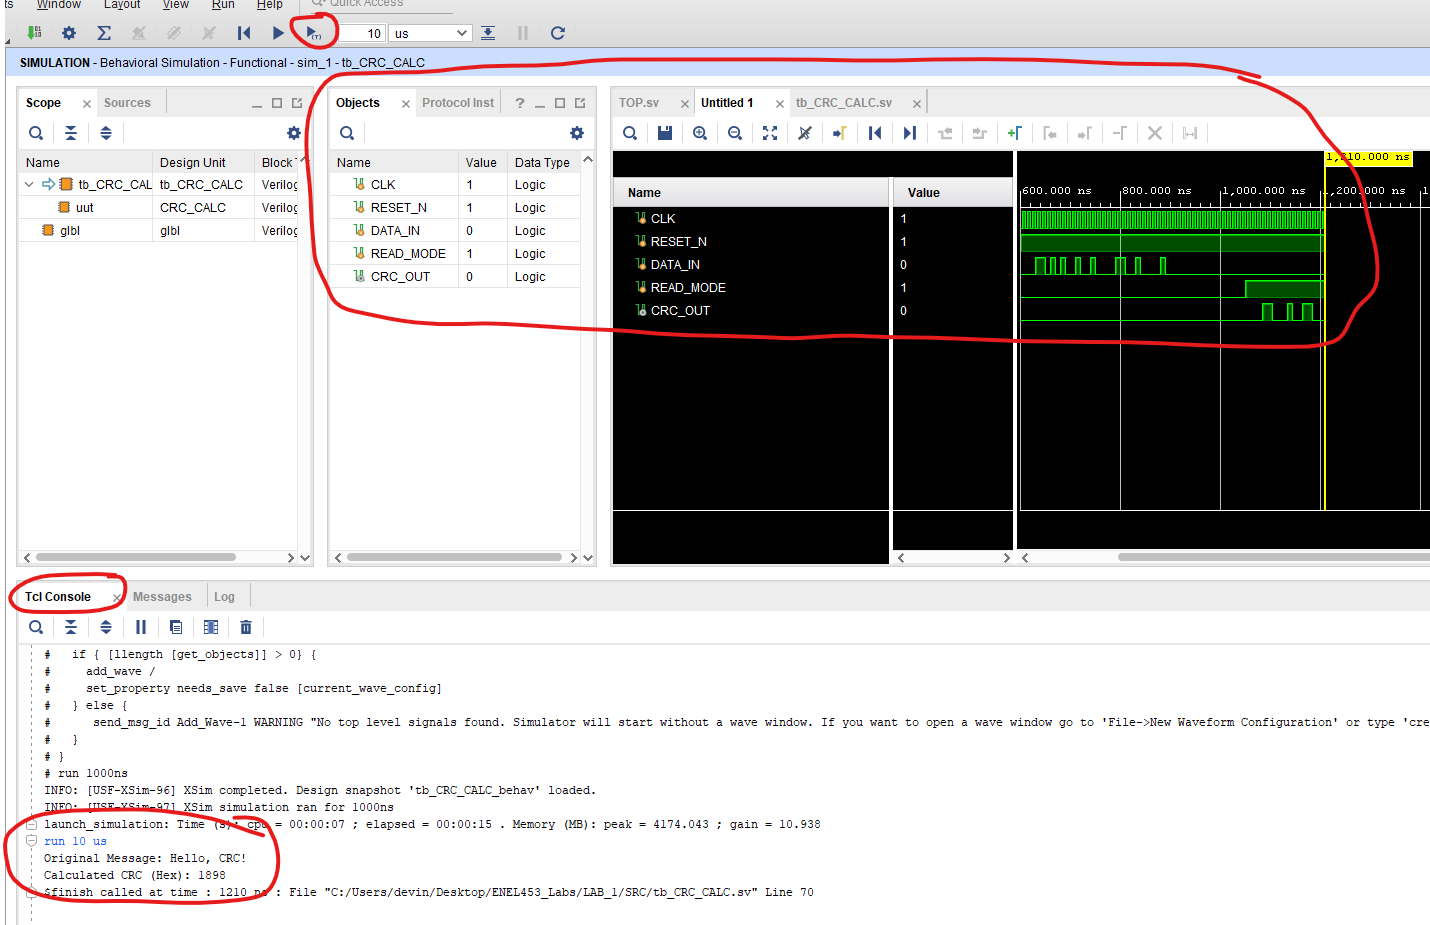
\includegraphics[width=7cm]{Images/SimulatingDesign/Run_Simulation_Page2.png}
    \caption{Your Simulation should run}
    \label{fig:enter-label}
\end{figure}
The simulation will run for a short time and then stop part way. Click the button up at the top next to the play button to run for an additional 10\begin{math}\mu\end{math}s. This will run the simulation through calculating the CRC value. In the large window you will be able to see the different signals changing over time. If you select the TCL console you will see that your simulation printed 2 lines of text.\\
\begin{verbatim}
    Original Message: Hello, CRC!
    Calculated CRC (Hex): 1898
\end{verbatim}
You can calculate the XMODEM CRC check value for the text and you'll find the value is correct for the input text. 
\subsection{Modifications}
\subsubsection{Adjusting Reset}
Open top\_level.sv. The provided code uses an active low reset; however, the button on the Basys3 board which it is hooked up to is active high.\\
\begin{itemize}
    \item \textbf{Modify the reset polarity in the code}. When you reprogram the board the LEDs should show up without needing to press the center button on the Basys3. 
\end{itemize}


To add the inverter look first at the top level of the design first look at the first at the top level of the design. 
\begin{lstlisting}
    module top_level (
    input CLK,
    input |\colorbox{magenta!30}{RESET}|,
    input [15:0] SWITCHES,
    output [15:0] LEDS
);
 
    // CRC Output Signal
    logic CRC_OUT;

    // Data Input Signal for CRC Calculation
    reg DATA_IN;
    
    // Read Mode Signal
    reg READ_MODE;

    // CRC Module Instance
    CRC_CALC crc_calc (
        .CLK(CLK),
        .|\colorbox{magenta!30}{RESET\_N(RESET)}|,
        .DATA_IN(DATA_IN),
        .READ_MODE(READ_MODE),
        .CRC_OUT(CRC_OUT)
    );

    // State Machine Instance
    CRC_Statemachine state_machine (
        .CLK(CLK),
        .|\colorbox{magenta!30}{RESET\_N(RESET)}|,
        .INPUT_CRC(SWITCHES),
        .OUTPUT_CRC(LEDS),
        .DATA_IN(DATA_IN),
        .READ_MODE(READ_MODE),
        .CRC_OUT(CRC_OUT)
    );

endmodule

\end{lstlisting}
Looking at the highlighted resets you can see that the top level reset is active high, while the lower level modules are active low. This means that the design is held in reset continually until reset is pressed where you will start to see outputs. To change this go into the lower level modules and adjust the resets to be active high. \textbf{\*Note that having a mix between RESET\_N and RESET hooking up in the way shown in the provided top module is bad practice, but was done here to demonstrate the mismatch in reset polarities.}\\
\vspace{0.5cm}
\begin{lstlisting}
    
module CRC_CALC(
    input CLK,
    input |\colorbox{magenta!30}{RESET}|,
    input DATA_IN,
    input READ_MODE,
    output reg CRC_OUT
    );
    
    // CRC Register
    reg [15:0] CRC_REG;
    
    // CRC Polynomial (XMODEM) 16'h1021
    
    // CRC Calculation
always @(posedge CLK) begin
    if (|\colorbox{magenta!30}{RESET}|) begin // Active Synchronous Reset
    
        CRC_REG <= 16'h0000; // Reset the CRC Register to 0
        CRC_OUT <= 1'b0; // Reset the CRC Output to 0
    end else if (READ_MODE) begin
        // Read Mode COde
    end else begin                                             
        // CRC Calculation Mode Code
        end
    end
 
endmodule

\end{lstlisting}
You can see required changes in the above code. The resets have been adjusted to reflect the need for active high reset on this hardware. You will need to perform these changes on your own code as well as similar changes to the crc state machine module and the associated test benches for each module. 


\subsubsection{Changing to a new CRC Calculation}
Open crc\_calc.sv. This implements a basic hardware design for performing 16-bit CRC calculations. Open the website: \url{https://crccalc.com/}, look at the 16-bit CRC calculations. Find the CRC-16/XMODEM and the CRC-16/CDMA2000 lines. Examine the differences between the different CRC checks.
\begin{itemize}
    \item \textbf{Adjust the initialization value of the CRC register to match the CRC-16/CDMA2000 standard}. You'll want to ensure you can simulate the original design first; however, you can use the provided website to check your answers.
    \item \textbf{Adjust the CRC Polynomial coded into the design to match the CRC-16/CDMA2000 standard}. Confirm that your output is as expected before submitting the design. A hand diagram can help immensely in ensuring that you don't make any mistakes
\end{itemize}
Look at the code in the CRC calculator module you can find code for resetting the CRC register as well as the code that represents the CRC polynomial.
\begin{lstlisting}
if (!RESET_N) begin        // Active Low Synchronous Reset
    |\colorbox{magenta!30}{CRC\_REG <= 16'h0000;}|     // Reset the CRC Register to 0
    CRC_OUT <= 1'b0;      // Reset the CRC Output to 0
end else if (READ_MODE) begin
            CRC_OUT <= CRC_REG[15];
            CRC_REG <= {CRC_REG[14:0], |\colorbox{magenta!30}{1'b0}|};
end else ...
\end{lstlisting}
The highlighted code resets the register to 0 when the module is reset. This aligns with the XMODEM standard. CDMA2000 gives the register an initial value of all ones. Adjust the code to meet the new standard. Remember to also adjust the value being pushed into the CRC register during read.\\
\vspace{0.5cm}
\begin{lstlisting}
CRC_REG[15] <= CRC_REG[14];
CRC_REG[14] <= CRC_REG[13];
CRC_REG[13] <= CRC_REG[12];
CRC_REG[12] <= |\colorbox{magenta!30}{CRC\_REG[11] {\^{}} CRC\_REG[15]}|;
CRC_REG[11] <= CRC_REG[10];
CRC_REG[10] <= CRC_REG[9];
CRC_REG[9] <= CRC_REG[8];
CRC_REG[8] <= CRC_REG[7];
CRC_REG[7] <= CRC_REG[6];
CRC_REG[6] <= CRC_REG[5];
CRC_REG[5] <= |\colorbox{magenta!30}{CRC\_REG[4] {\^{}} CRC\_REG[15]}|;
CRC_REG[4] <= CRC_REG[3];
CRC_REG[3] <= CRC_REG[2];
CRC_REG[2] <= CRC_REG[1];
CRC_REG[1] <= CRC_REG[0];
CRC_REG[0] <= |\colorbox{magenta!30}{CRC\_REG[15] {\^{}} DATA\_IN}|;
\end{lstlisting}

This chunk of code is provided for you. You can see overall that it takes the general form of a shift register where each clock cycle shifts the bits over by 1 through the register; however, bit 12, 5, and 0 are different. These are implementing the CRC Polynomial 0x1021 which may also be represented by \(x^{15} + x^{12} + x^{5} + 1\). You can see that the 12th bit, 5th bit, and 0th bit are each exclusively or-ed with the 15th bit when shifting over. Modify the code to match the CRC polynomial of the CDMA2000 standard which is \(x^{15}+x^{14}+x^{11}+x^{6}+x^5 + x^2 +x^1 + 1\). You can copy the pattern from the XMODEM implementation to create an equivalent CDMA2000 implementation.\\
\vspace{0.5cm}
\textbf{Do not modify the provided module headers. Your submitted files will be tested against a series of randomized cases to verify that they perform correctly.}


\section{Create Bitstream (In the Lab)}
\ifpdf

    \vspace{1cm}
    \begin{figure}[H]
        \centering
        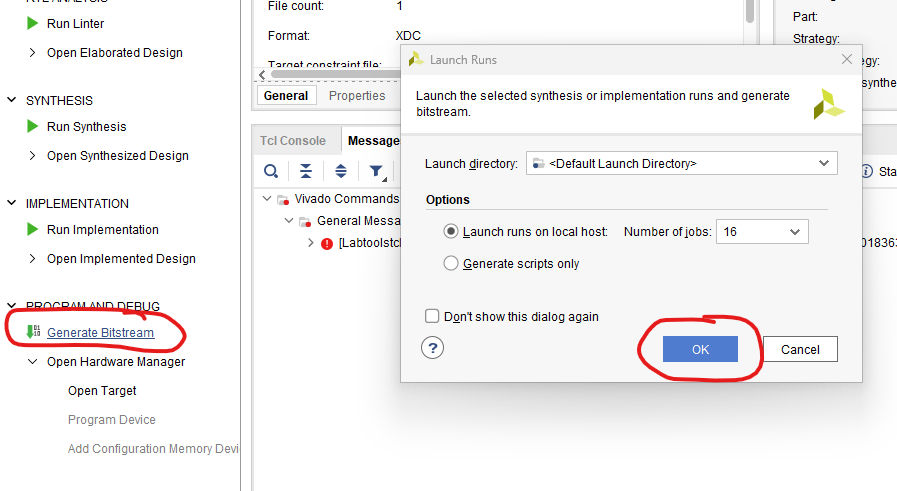
\includegraphics[width=9cm]{Images/CreateBitstreamImages/Vivado_GenerateBitstream.png}
        \caption{Click on Generate Bitstream}
        \label{fig:enter-label}
        \raggedright
        \vspace{0.5cm}
        When creating your own files you will need to simulate each file before attempting to upload it to the board. In this particular case we have validated the provided files to ensure that they work on the Basys 3 boards, so you could have clicked directly on "Generate\_Bitstream" without stepping through synthesis and implementation independently. Assuming your design sources and constraints are correctly set it should begin generating a bitstream file for the Basys 3. You can increase the number of jobs to save some time. 

    \end{figure}

    \begin{figure}[H]
        \centering
        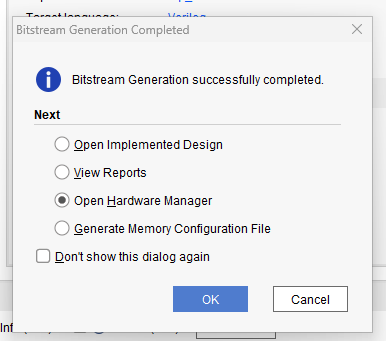
\includegraphics[width=9cm]{Images/CreateBitstreamImages/Vivado_BitstreamGenerated.png}
        \caption{Select Open Hardware Manager}
        \label{fig:enter-label}
    \end{figure}
    Once the bitstream is completed a box will pop up. Ensure that open hardware manager is selected, then hit okay.

    \begin{figure}[H]
        \centering
        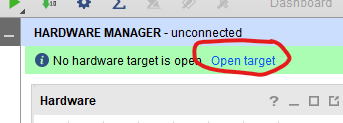
\includegraphics[width=9cm]{Images/CreateBitstreamImages/Vivado_OpenTarget.png}
        \caption{Select Open Target and hit Auto Connect}
        \label{fig:enter-label}
    \end{figure}
    This will begin the connection to the the local hardware server which Xilinx uses to talk with the Basys 3 board. If you were using a remote board then you will need to set the server IP. 
    
    \begin{figure}[H]
        \centering
        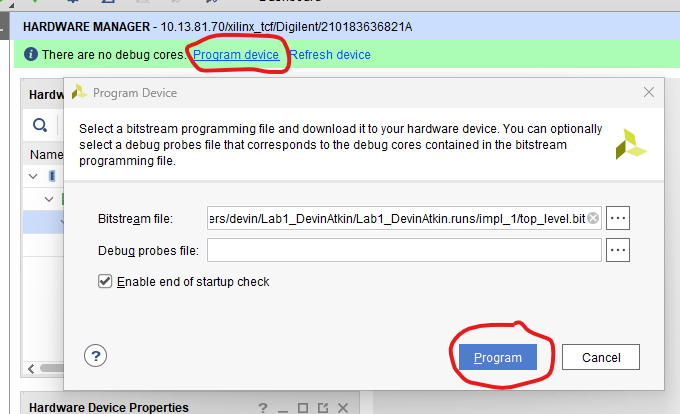
\includegraphics[width=9cm]{Images/CreateBitstreamImages/Vivado_ProgramHardware.png}
        \caption{Select Program Device}
        \label{fig:enter-label}
    \end{figure}
    Once connected you should select program device and then hit program. This should send the generated bitstream to the Xilinx hardware. Assuming no errors come up, then you should be able to tell if the programming worked by Green done LED turning on. 
\else
    \HCode{<video width="320" height="240" controls>
    <source src="Images/CreateProject_Vivado2023.mp4" type="video/mp4">
    <img src="Images/Vivado_CreateProject.png" alt="Video Shows the button press for the create project">
    Your browser does not support the video tag. (Still need to update this to a new video)
    </video>}
\fi
Your marks are split evenly between your code and the explainer video.\\
\begin{itemize}
    \item Include all the required files for your design and test benches. This means that all the System Verilog Files are present even if they are unmodified. Also be sure to include the associated constraints file.
    \item Ensure the provided code produces an led pattern at a speed which is clear at human time-scales. 
    \item Include a design report file. This should include your timing constraints and a calculation of the maximum operating frequency for your design. It also needs to include a screenshot of your RTL view after making the modifications. Your report should have a cover page containing your Name, Student ID, Lab Section, and Lab Title. 
    \item \textbf{Create a timing diagram showing pulse width modulation and explaining why it can be used to produce a dimming effect with LEDs. Include this in your design report alongside the other material}. Feel free to use tools like  \url{https://wavedrom.com/} to produce your timing diagrams. If using one of these tools make sure to include the text used to generate the waveform diagram. 
    \item Record a short 1-3 minute video explaining what you have done. Look at each segment of your code and explain approximately how it is working. 
\end{itemize}

\vspace{0.5cm}
Provide a video of you walking through each section of your code and explaining your reasoning. Your video should be no more than 4 minutes long. Ensure that you are clearly audible through the video. 
\end{document}
